
\section{Παραλλαγή του Logistic Χάρτη}


Μελετήθηκε η δυναμική συμπεριφορά της εξίσωσης διακριτού χρόνου:

	\begin{equation}
		x_i=k*(a+x_{i-1})^2 *(b-x_{i-1}))
		\label{f:x1}
	\end{equation}


	όπου a,b,k, q:παράμετροι\\\\
	
	Για την εύρεση της δυναμικής συμπεριφοράς του συστήματος εξετάστηκε μια περιοχή τιμών των συγκεκριμένων παραμέτρων, ώστε να επιτευχθεί ταυτόχρονη σύγκριση της περιοδικής και χαοτικής συμπεριφοράς του. Πιο συγκεκριμένα, στη μελέτη που πραγματοποιήθηκε οι παράμετροι a, b, κρατήθηκαν αρχικά σταθερές με τιμές a=1, b=2  όπως και η αρχική συνθήκη του x1 =0.1 παρέμεινε  σταθερή,  ενώ η τιμή της παραμέτρου q μεταβάλλονταν στο διάστημα[0.1,1.7] με βήμα 0.2. Έτσι, για κάθε περίπτωση παράχθηκαν το διάγραμμα διακλάδωσης, ο εκθέτης Lyapunov και το διάγραμμά της τιμής xi σε συνάρτηση με την τιμή xi-1., τα οποία παρουσιάζονται και αναλύονται στη συνέχεια.
	
\subsection{Για q=-0.1}


	
Στο σχήμα \ref{f:g1} παρατίθεται το διάγραμμα διακλάδωσης του συστήματος \ref{f:x1}, ως προς την παράμετρο k, για a=1, b=2 και q =- 0.1. Για αυτές τις τιμές των παραμέτρων το σύστημα ξεκινάει από περίοδο-1 για k = 0.3 , ενώ για  k = 0.4 εμφανίζει τον πρώτο διπλασιασμό της περιόδου. Τον δεύτερο διπλασιασμό τον εμφανίζει για k=0.47 (περίοδος-4) ,τον τρίτο για k=0.476(περίοδος-8) . Ενώ ο τελευταίος διπλασιασμός εμφανίζεται λίγο πιο μετά τον τρίτο για k=0.478 (περίοδος-16). Στην συνέχεια για k>0.479το σύστημα εισέρχεται στο χάος , μέχρι να εξέλθει  για k=0.51(περίοδος-3) και να ξανά εισέλθει σε χάος μετά από δύο διπλασιασμούς k=0.52(περίοδος-6) και k=0.522(περίοδος-11) για k>0.524. To φαινόμενο αυτό είναι γνωστό ως συνοριακή κρίση .Εξέρχεται για τελευταία φορά από το χάος για k=0.555 (περίοδος-4). Για k=0.559 εμφανίζεται ένας διπλασιασμός (περίοδος-8) ο οποίος καταστρέφεται για k=0.567 , οπότε εδώ παρατηρούμε αντιμονοτονικότητα δηλαδή έχουμε μία ανάστροφη ακολουθία διπλασιασμού της περιόδου για k=0.568. Λόγω αυτού του φαινομένου το οποίο συνεχίζει μέχρι το q=-0.2,μελετήθηκε περαιτέρω το σύστημα από -0.1<q<-0.2.Τέλος για k=0.5735 έχουμε έναν τελευταίο διπλασιασμό(περίοδος-6) πριν ξανά εισέλθει το σύστημα για k>0.575 στο χάος.
Στο σχήμα \ref{f:g2} παρατίθενται 3 διαγράμματα διακλάδωσης \ref{f:g3}, \ref{f:g4}, \ref{f:g5}, \ref{f:g6}
για 0.54<k<0.6. Ουσιαστικά εστιάστηκε το διάγραμμα στην αντιμονοτονικότητα που εμφανίζεται για τις συγκεκριμένες τιμές του q. Επίσης παρατηρούμε στα διαγράμματα \ref{f:g4}, \ref{f:g5}, \ref{f:g6} δημιουργία χαοτικών φυσαλίδων. Δηλαδή, το σύστημα εισέρχεται στο χάος με διπλασιασιασμό της περιόδου και στην συνέχεια εξέρχεται από αυτό με αντίστροφο διπλασιασμό της περιόδου. Επιπλέον στο διάγραμμα \ref{f:g6} το φαινόμενο εμφανίζεται δυο φορές  για 0.560<k<0.568 και 0.571<k<0.573. 
Επιπλέον, στο σχήμα \ref{f:g7} παρατίθεται το διάγραμμα των εκθετών Lyapunov για τιμές του k στο ίδιο διάστημα τιμών [0.3, 0.6].  Στο διάστημα τιμών   k=0.522 , στο 0.51<k<0.522, και στο 0.554<k<0.574 παρατηρούμε ότι ο εκθέτης Lyapunov είναι συνεχώς αρνητικός, γεγονός που επιβεβαιώνει την περιοδική συμπεριφορά του συστήματος. Ενώ στα υπόλοιπα διαστήματα ο θετικός εκθέτης Lyapunov υποστηρίζει την χαοτική του συμπεριφορά, όπως έγινε φανερό και από το διάγραμμα διακλάδωσης.
Τέλος, στον Πίνακα \ref{tab:abc} παρατίθενται ενδεικτικές τιμές της παραμέτρου k και η συμπεριφορά που παρουσιάζει το σύστημα για αυτές, σύμφωνα με το διάγραμμα διακλάδωσης, καθώς και τα αντίστοιχα σχήματα των διαγραμμάτων της τιμής \(x_i\) σε συνάρτηση με την τιμή \(x_{i+1}\). Από τα παραγόμενα σχήματα προκύπτει αριθμός σημείων αντίστοιχος με την περίοδο του συστήματος.


\begin{table}[h!]
	\centering
	\begin{tabular}{l | l | l}
		Παράμετρος k & Συμπεριφορά & Σχήμα\\
		\hline
		0.3 &  Περίοδος-1 & \ref{f:k1}\\
		0.41 & Περίοδος-2 & \ref{f:k2}\\
		0.476 &  Περίοδος-8 & \ref{f:k3}\\
		0.4778 & Περίοδος-16 & \ref{f:k4}\\
		0.479 & Χάος & \ref{f:k5}\\
		0.517 & Περίοδος-3 & \ref{f:k6})\\
		0.52 & Περίοδος-6 & \ref{f:k7}\\
		0.522 & Περίοδος-11 & \ref{f:k8}\\
		0.524 & Χάος & \ref{f:k9}\\
		0.555 & Περίοδος-4 & \ref{f:k10}\\
		0.559 & Περίοδος-8 & \ref{f:k11}\\
		0.568 & Περίοδος-4 & \ref{f:k12}\\
		0.5735 & Περίοδος-6 & \ref{f:k13}\\
		0.575 & Χάος & \ref{f:k14}\\
	\end{tabular}
	\caption{ Συμπεριφορά του υπό μελέτη συστήματος για διάφορες τιμές του k,για a=1, b=2 και q=-0.1}
	\label{tab:abc}
\end{table}


\begin{figure}[h!]
	\centering
	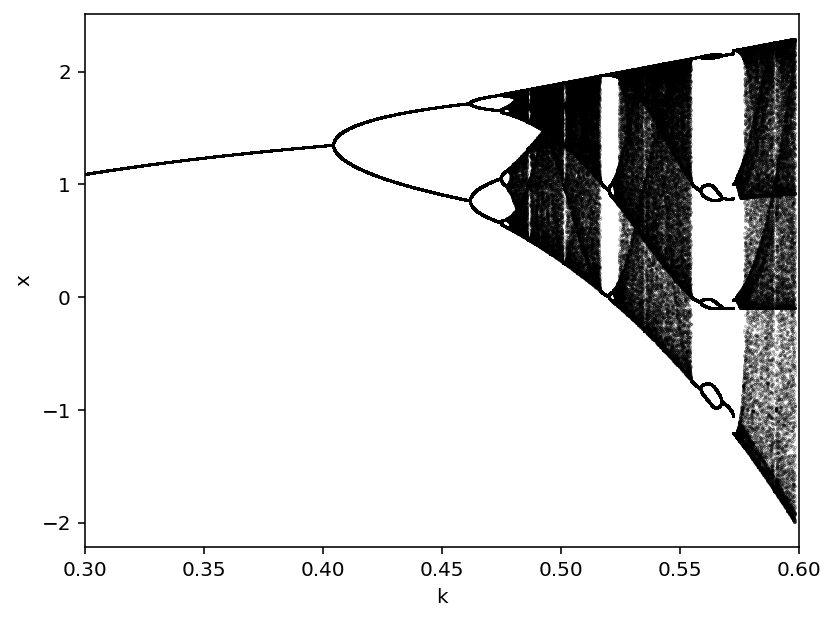
\includegraphics[width=0.6\linewidth]{LateX images/graphs/g1}
	\caption{ Διάγραμμα διακλάδωσης, για a=1, b=2 και q=-0.1}
	\label{f:g1}
\end{figure}



\begin{figure}[h!]
	\centering
	\caption{}
	\label{f:g2}
	\begin{subfigure}[b]{0.4\textwidth}
		\centering
		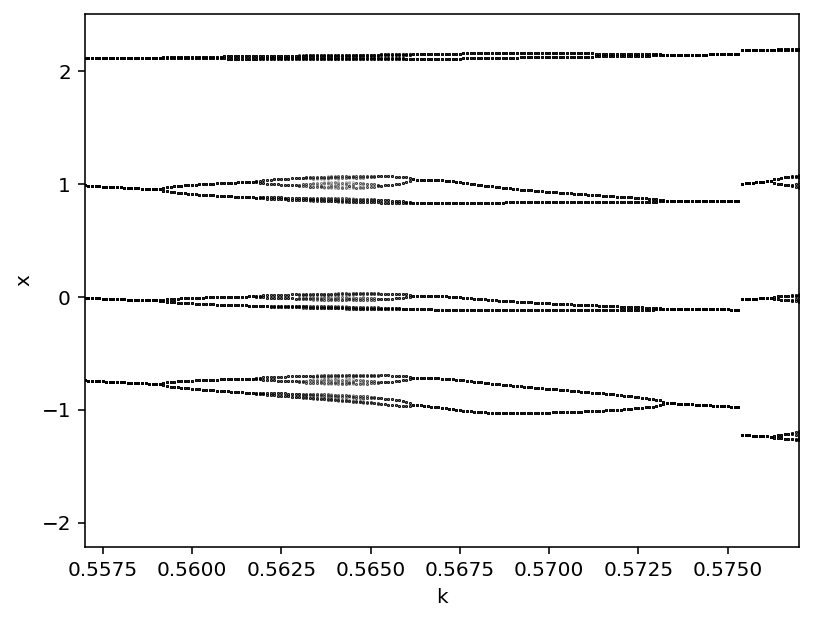
\includegraphics[width=\textwidth]{LateX images/graphs/g2}
		\caption{Διάγραμμα διακλάδωσης, για q=-0.112}
		\label{f:g3}
	\end{subfigure}
	\hfill
	\begin{subfigure}[b]{0.4\textwidth}
		\centering
		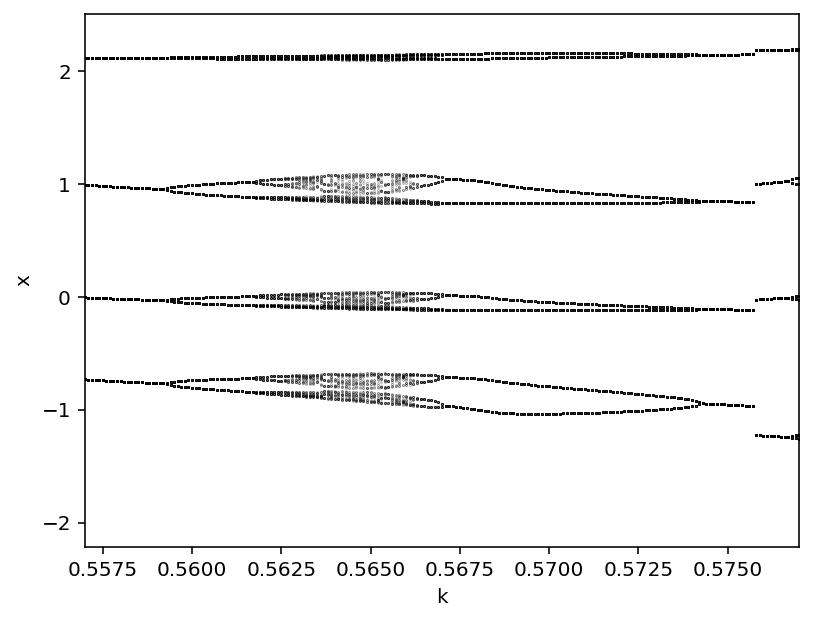
\includegraphics[width=\textwidth]{LateX images/graphs/g3}
		\caption{Διάγραμμα διακλάδωσης, για q=-0.114}
		\label{f:g4}
	\end{subfigure}
	\hfill
	\begin{subfigure}[b]{0.4\textwidth}
		\centering
		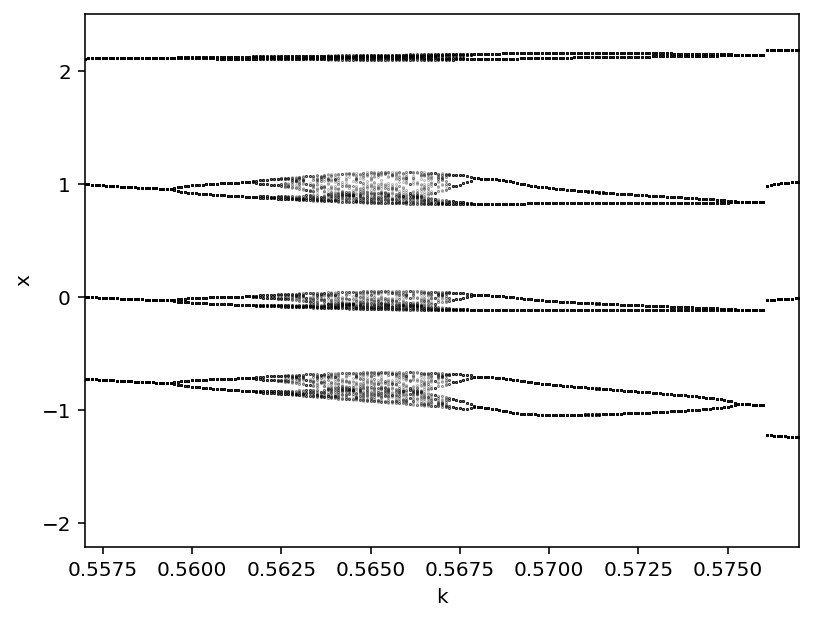
\includegraphics[width=\textwidth]{LateX images/graphs/g4}
		\caption{Διάγραμμα διακλάδωσης, για q=-0.116}
		\label{f:g5}
	\end{subfigure}
	\hfill
	\begin{subfigure}[b]{0.4\textwidth}
		\centering
		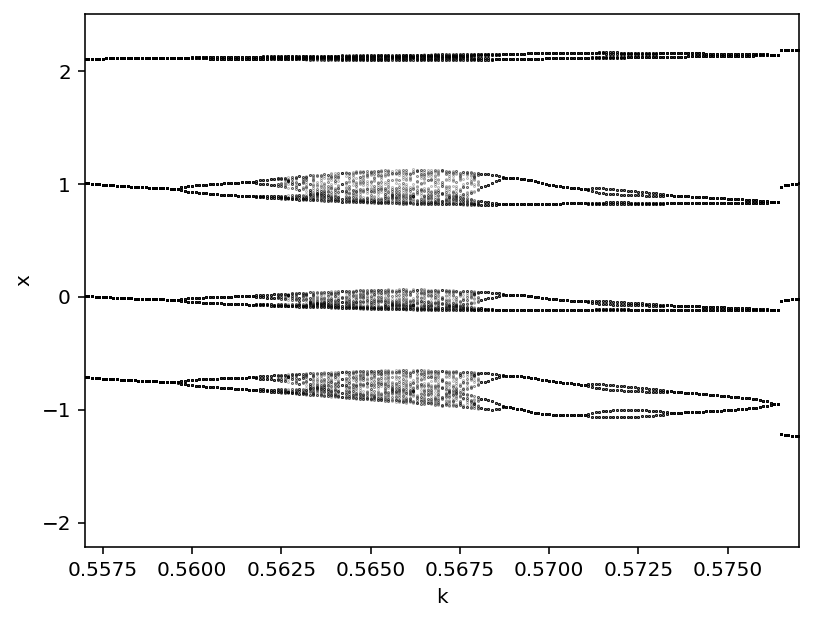
\includegraphics[width=\textwidth]{LateX images/graphs/g5}
		\caption{Διάγραμμα διακλάδωσης, για q=-0.118}
		\label{f:g6}
	\end{subfigure}
\end{figure}

\begin{figure}[h!]
	\centering
	\includegraphics[width=0.6\linewidth]{"LateX images/graphs/g6 "}
	\caption{Διάγραμμα του εκθέτη Lyapunov σε συνάρτηση με την παράμετρο k, για a=1, b=2 και q=-0.1.}
	\label{f:g7}
\end{figure}



\begin{figure}[h!]
	\centering
	\caption{Διαγράμματα της τιμής \(x_i\) με την τιμή \(x_{i+1}\) :}
	\begin{subfigure}[b]{0.25\textwidth}
		\centering
		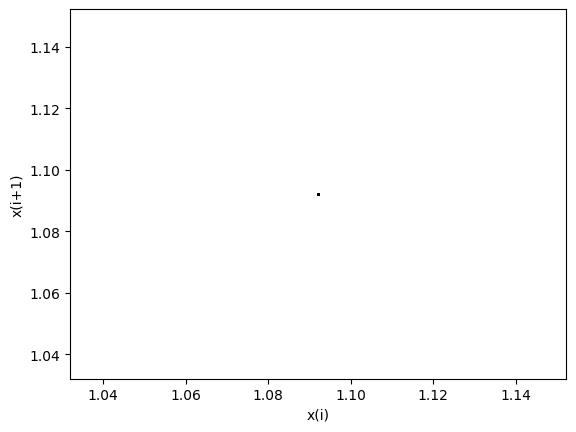
\includegraphics[width=\textwidth]{LateX images/graphs/k03}
		\caption{Για k=0.3}
		\label{f:k1}
	\end{subfigure}
	\hfill
	\begin{subfigure}[b]{0.25\textwidth}
		\centering
		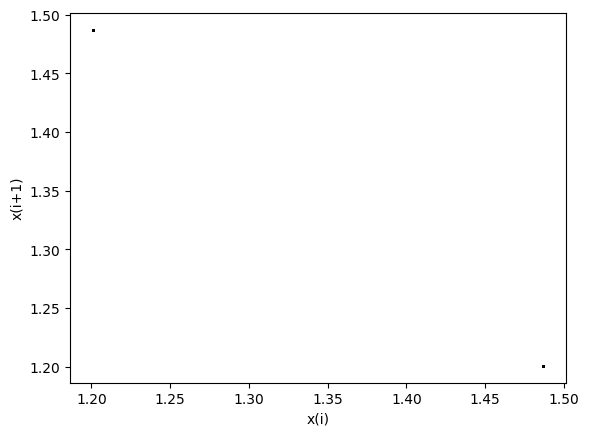
\includegraphics[width=\textwidth]{LateX images/graphs/k041}
		\caption{Για k=0.41}
		\label{f:k2}
	\end{subfigure}
	\hfill
	\begin{subfigure}[b]{0.25\textwidth}
		\centering
		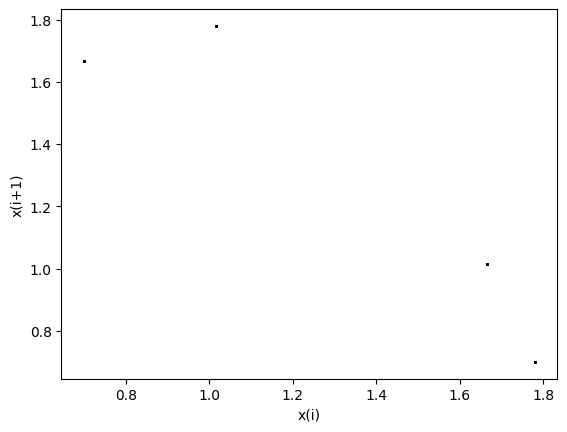
\includegraphics[width=\textwidth]{LateX images/graphs/k047}
		\caption{Για k=0.047}
		\label{f:k3}
	\end{subfigure}
	\begin{subfigure}[b]{0.25\textwidth}
		\centering
		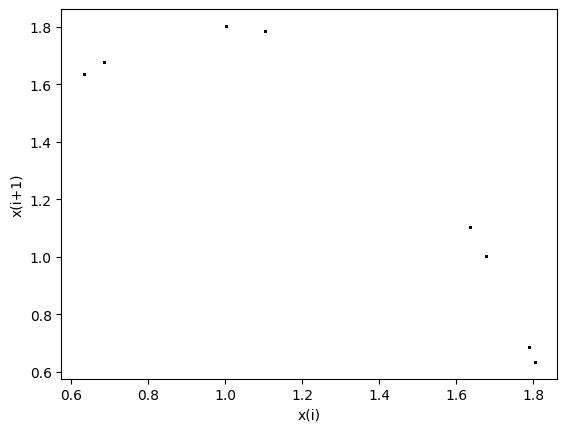
\includegraphics[width=\textwidth]{LateX images/graphs/k0476}
		\caption{Για k=0.476}
		\label{f:k4}
	\end{subfigure}
	\hfill
	\begin{subfigure}[b]{0.25\textwidth}
		\centering
		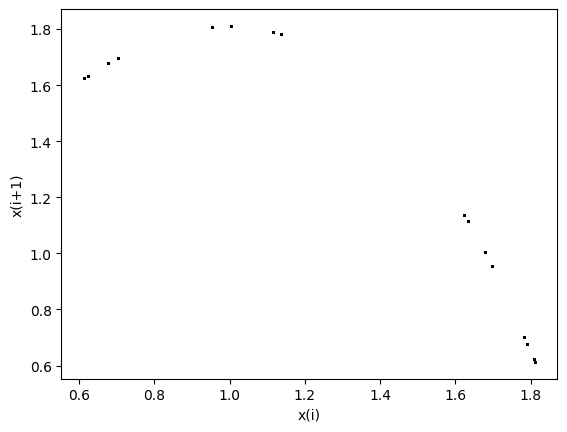
\includegraphics[width=\textwidth]{LateX images/graphs/k04778}
		\caption{Για k=0.4778}
		\label{f:k5}
	\end{subfigure}
	\hfill
	\begin{subfigure}[b]{0.25\textwidth}
		\centering
		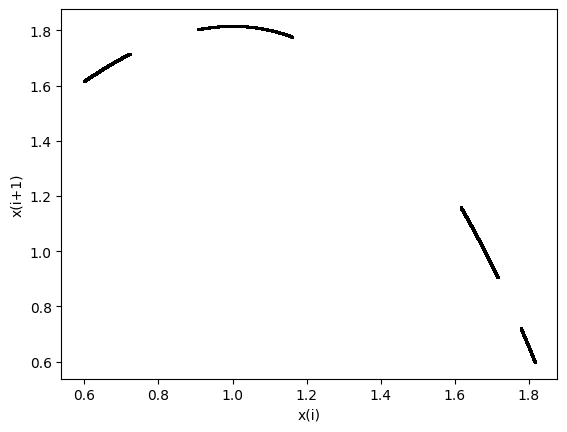
\includegraphics[width=\textwidth]{LateX images/graphs/k0479}
		\caption{Για k=0.479}
		\label{f:k6}
	\end{subfigure}
	\hfill
	\begin{subfigure}[b]{0.25\textwidth}
		\centering
		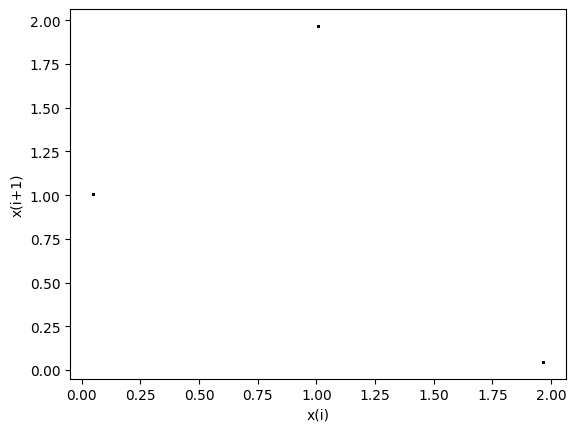
\includegraphics[width=\textwidth]{LateX images/graphs/k0517}
		\caption{Για k=0.517}
	\end{subfigure}
	\hfill
	\begin{subfigure}[b]{0.25\textwidth}
		\centering
		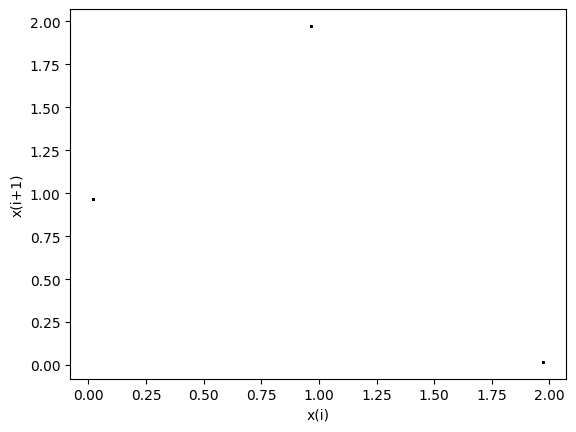
\includegraphics[width=\textwidth]{LateX images/graphs/k0519}
		\caption{Για k=0.519}
		\label{f:k7}
	\end{subfigure}
	\hfill
	\begin{subfigure}[b]{0.25\textwidth}
		\centering
		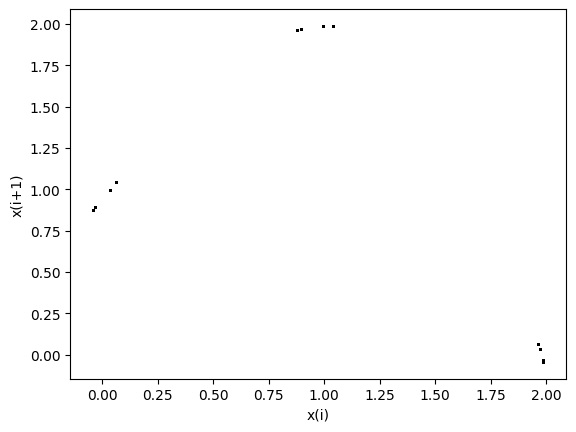
\includegraphics[width=\textwidth]{LateX images/graphs/k0522}
		\caption{Για k=0.522}
		\label{f:k8}
	\end{subfigure}
	\hfill
	\begin{subfigure}[b]{0.25\textwidth}
		\centering
		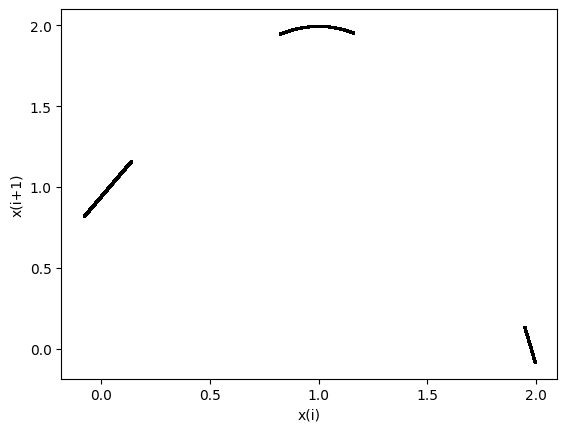
\includegraphics[width=\textwidth]{LateX images/graphs/k0524}
		\caption{Για k=0.524}
		\label{f:k9}
	\end{subfigure}
	\hfill
	\begin{subfigure}[b]{0.25\textwidth}
		\centering
		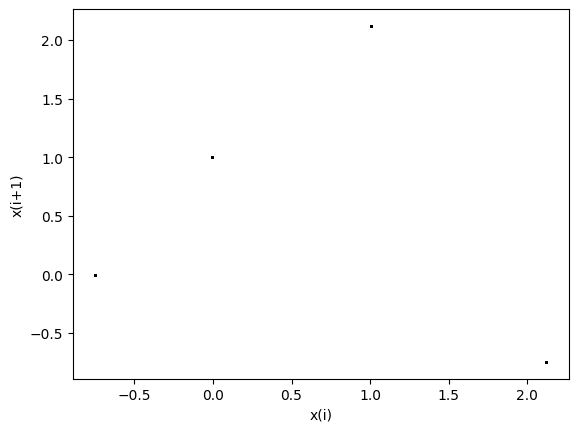
\includegraphics[width=\textwidth]{LateX images/graphs/k0555}
		\caption{Για k=0.555}
		\label{f:k10}
	\end{subfigure}
	\hfill
	\begin{subfigure}[b]{0.25\textwidth}
		\centering
		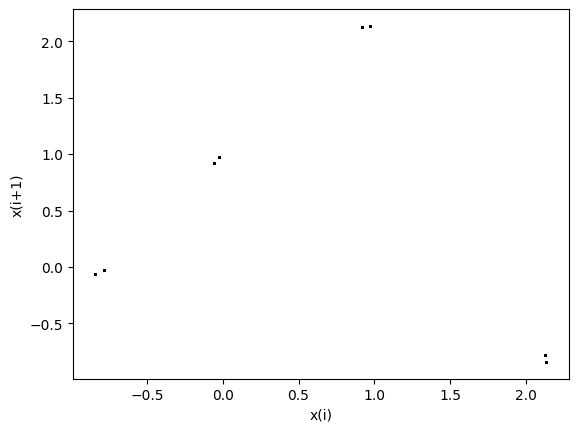
\includegraphics[width=\textwidth]{LateX images/graphs/k0559}
		\caption{Για k=0.559}
		\label{f:k11}
	\end{subfigure}
	\hfill
	\begin{subfigure}[b]{0.25\textwidth}
		\centering
		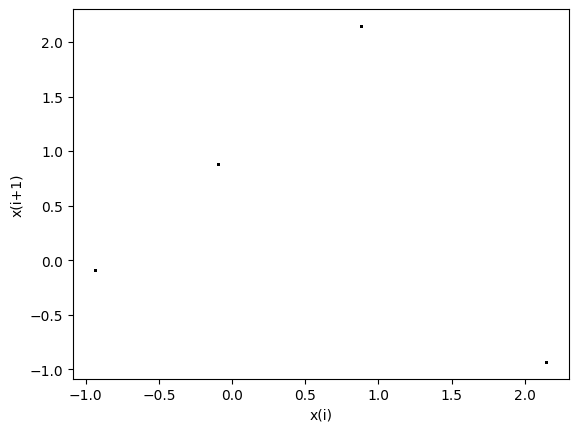
\includegraphics[width=\textwidth]{LateX images/graphs/k0568}
		\caption{Για k=0.568}
		\label{f:k12}
	\end{subfigure}
	\hfill
	\begin{subfigure}[b]{0.25\textwidth}
		\centering
		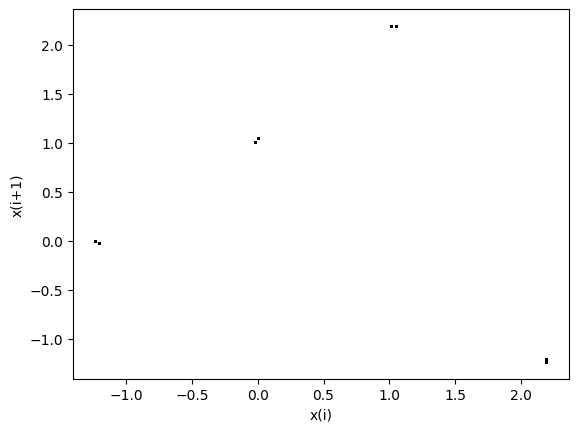
\includegraphics[width=\textwidth]{LateX images/graphs/k05735}
		\caption{Για k=0.5735}
		\label{f:k13}
	\end{subfigure}
	\hfill
	\begin{subfigure}[b]{0.25\textwidth}
		\centering
		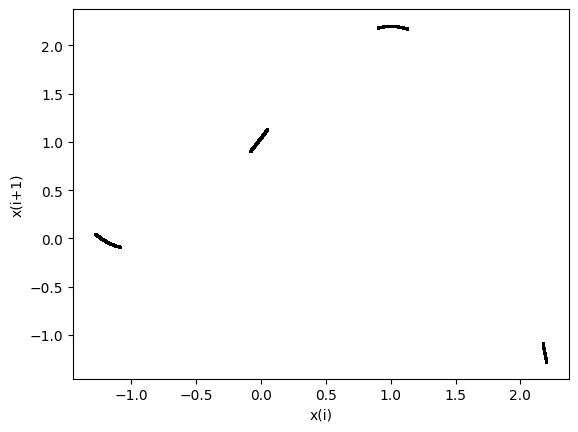
\includegraphics[width=\textwidth]{LateX images/graphs/k0575}
		\caption{Για k=0.575}
		\label{f:k14}
	\end{subfigure}

\end{figure}

 \clearpage
\subsection{Για q=-0.3}

Στο σχήμα \ref{f:g8} παρατίθεται το διάγραμμα διακλάδωσης του συστήματος \ref{f:x1}, ως προς την παράμετρο k, για a=1, b=2 και q =- 0.3. Για αυτές τις τιμές των παραμέτρων το σύστημα ξεκινάει από περίοδο-1 για k = 0.3 , ενώ για  k = 0.44 εμφανίζει τον πρώτο διπλασιασμό της περιόδου. Τον δεύτερο διπλασιασμό τον εμφανίζει για k=0.5 (περίοδος-4) ,τον τρίτο για k=0.511(περίοδος-8).Στην συνέχεια για k>0.5165 το σύστημα εισέρχεται στο χάος , μέχρι να εξέλθει  για k=0.551(περίοδος-3) και να ξανά εισέλθει σε χάος μετά από δύο διπλασιασμούς k=0.555(περίοδος-6) και k=0.556(περίοδος-12) για k>0.5573. To φαινόμενο αυτό είναι γνωστό ως συνοριακή κρίση .Εξέρχεται για τελευταία φορά από το χάος για k=0.583 (περίοδος-4) και μετά απο ένα διπλασιασμό  για k=0.5846(Περίόδος-7) είσέρχεται για τελευταία φορά στο χάος για k=0.5851.
Επομένως και σε αυτή την περίπτωση το σύστημα εισέρχεται στο χάος με διπλασιασμό της περιόδου. 
Επιπλέον, στο σχήμα \ref{f:g9} παρατίθεται το διάγραμμα των εκθετών Lyapunov για τιμές του k στο ίδιο διάστημα τιμών [0, 0.63].  Στο διάστημα τιμών   0<k<0.511 , στο 0.551<k<0.556, και στο 0.583<k<0.5846 παρατηρούμε ότι ο εκθέτης Lyapunov είναι συνεχώς αρνητικός, γεγονός που επιβεβαιώνει την περιοδική συμπεριφορά του συστήματος. Ενώ στα υπόλοιπα διαστήματα ο θετικός εκθέτης Lyapunov υποστηρίζει την χαοτική του συμπεριφορά, όπως έγινε φανερό και από το διάγραμμα διακλάδωσης.
Τέλος, στον Πίνακα \ref{tab:abc1} παρατίθενται ενδεικτικές τιμές της παραμέτρου k και η συμπεριφορά που παρουσιάζει το σύστημα για αυτές, σύμφωνα με το διάγραμμα διακλάδωσης, καθώς και τα αντίστοιχα σχήματα των διαγραμμάτων της τιμής \(x_i\) σε συνάρτηση με την τιμή \(x_{i+1}\). Από τα παραγόμενα σχήματα προκύπτει αριθμός σημείων αντίστοιχος με την περίοδο του συστήματος.
\begin{table}[h!]
	\centering
	\begin{tabular}{l | l | l}
		Παράμετρος k & Συμπεριφορά & Σχήμα\\
		\hline
		0.3 &  Περίοδος-1 & \ref{f:k1}\\
		0.44& Περίοδος-2 & \ref{f:k2}\\
		0.5& Περίοδος-4 & \ref{f:k2}\\
		0.511 &  Περίοδος-8 & \ref{f:k3}\\
		0.5165 & Χάος & \ref{f:k5}\\
		0.551 & Περίοδος-3 & \ref{f:k6})\\
		0.555 & Περίοδος-6 & \ref{f:k7}\\
		0.556 & Περίοδος-12 & \ref{f:k8}\\
		0.5573 & Χάος & \ref{f:k9}\\
		0.583& Περίοδος-4 & \ref{f:k10}\\
		0.5846 & Περίοδος-7 & \ref{f:k11}\\
		0.5851 & Χάος & \ref{f:k14}\\
	\end{tabular}
	\caption{ Συμπεριφορά του υπό μελέτη συστήματος για διάφορες τιμές του k,για a=1, b=2 και q=-0.3}
	\label{tab:abc1}
\end{table}

\begin{figure}[h!]
	\centering
	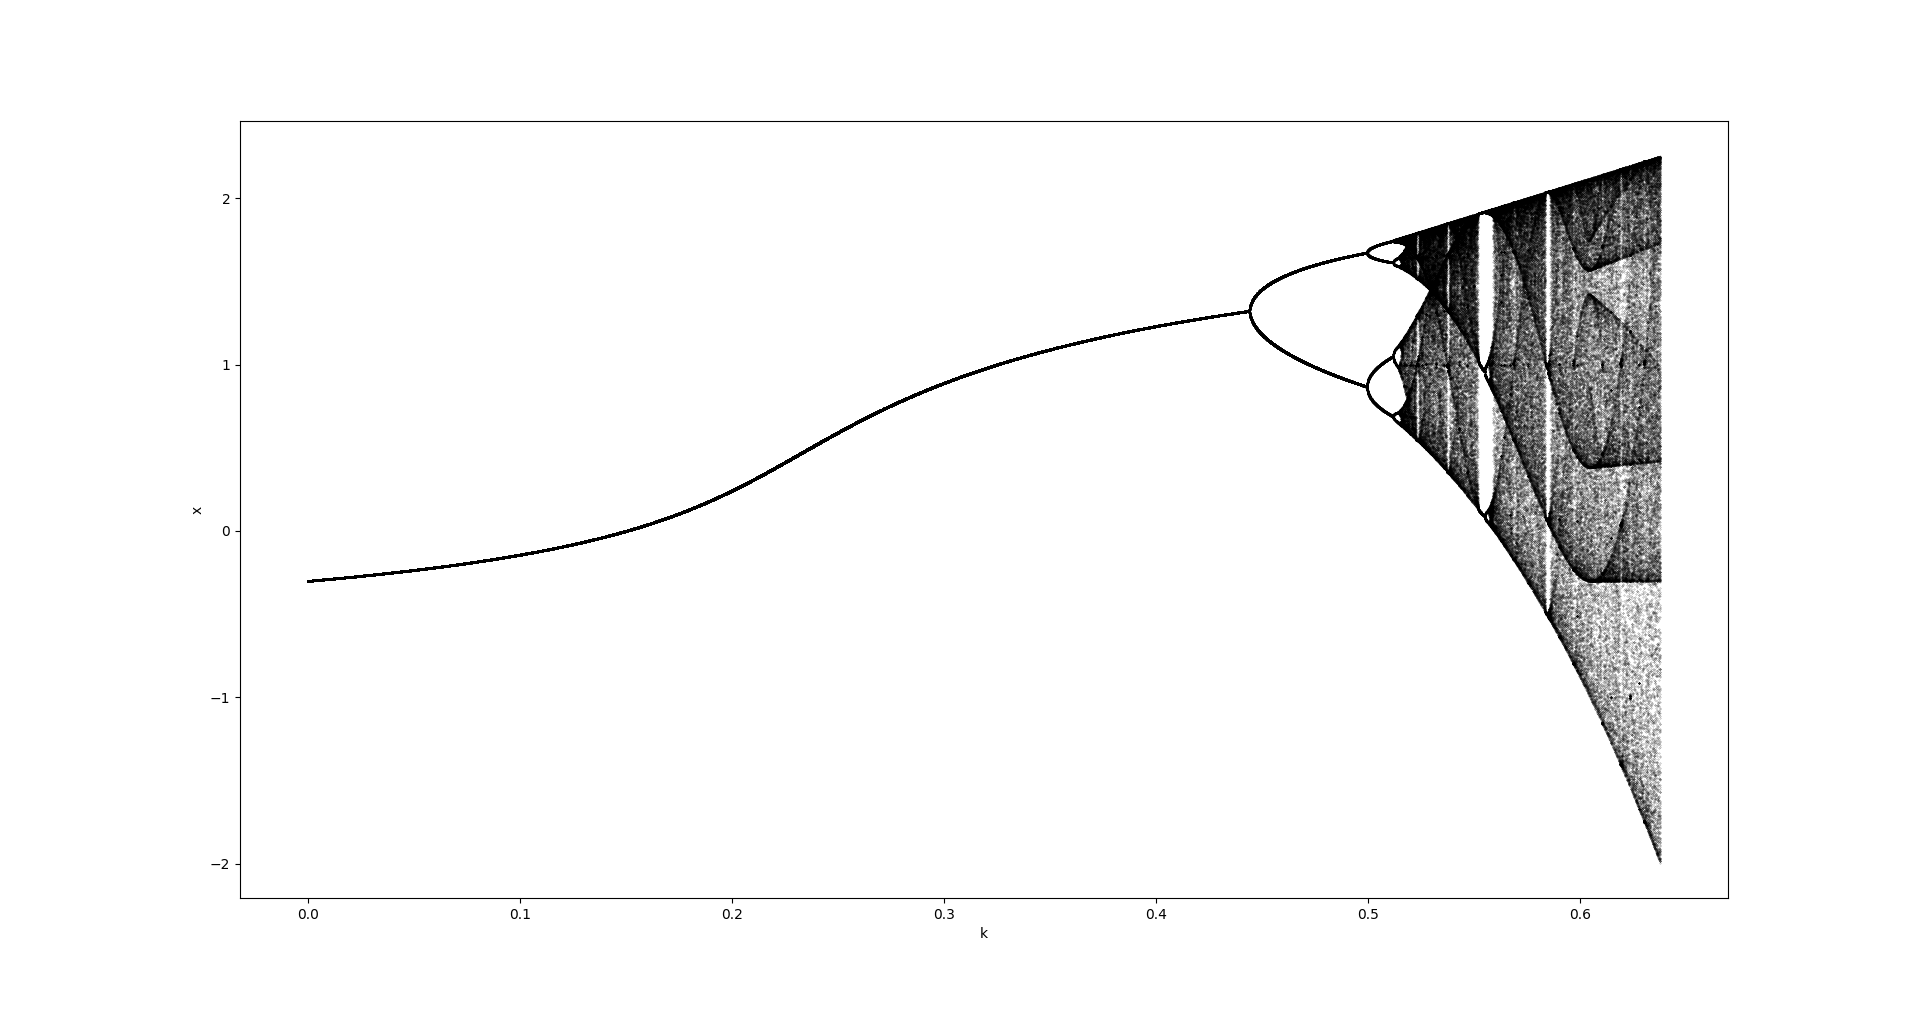
\includegraphics[width=0.6\linewidth]{LateX images/graphs q03/g1}
	\caption{ Διάγραμμα διακλάδωσης, για a=1, b=2 και q=-0.3}
	\label{f:g8}
\end{figure}

\begin{figure}[h!]
	\centering
	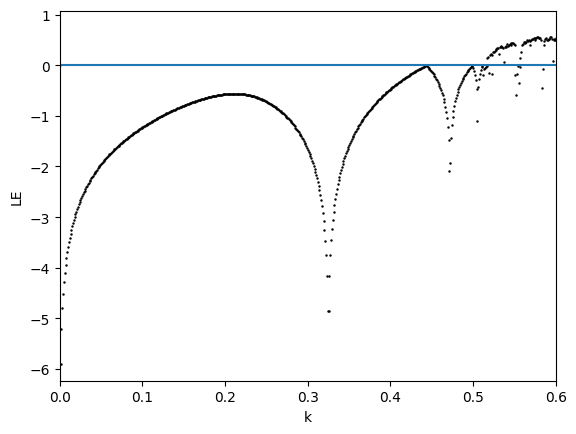
\includegraphics[width=0.6\linewidth]{LateX images/graphs q03/g2}
	\caption{ Διάγραμμα του εκθέτη Lyapunov σε συνάρτηση με την παράμετρο k, για a=1, b=2 και q=-0.3}
	\label{f:g9}
\end{figure}

\begin{figure}[h!]
	\centering
	\caption{Διαγράμματα της τιμής \(x_i\) με την τιμή \(x_{i+1}\) :}
	\begin{subfigure}[b]{0.25\textwidth}
		\centering
		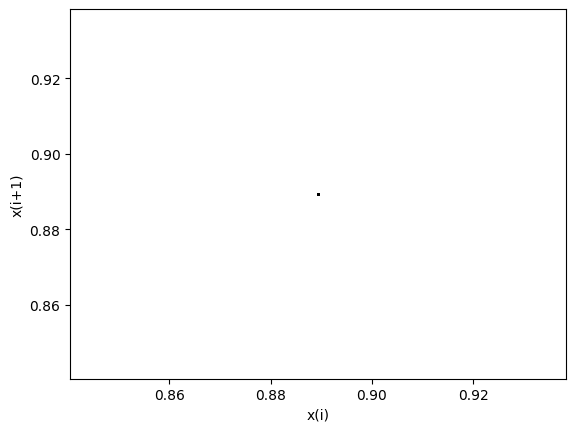
\includegraphics[width=\textwidth]{LateX images/graphs q03/g3}
		\caption{Για k=0.3}
		\label{f:k15}
	\end{subfigure}
	\hfill
	\begin{subfigure}[b]{0.25\textwidth}
		\centering
		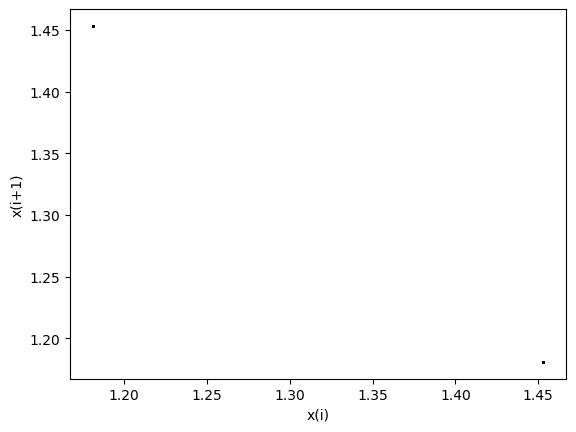
\includegraphics[width=\textwidth]{LateX images/graphs q03/g4}
		\caption{Για k=0.44}
		\label{f:k16}
	\end{subfigure}
	\hfill
	\begin{subfigure}[b]{0.25\textwidth}
		\centering
		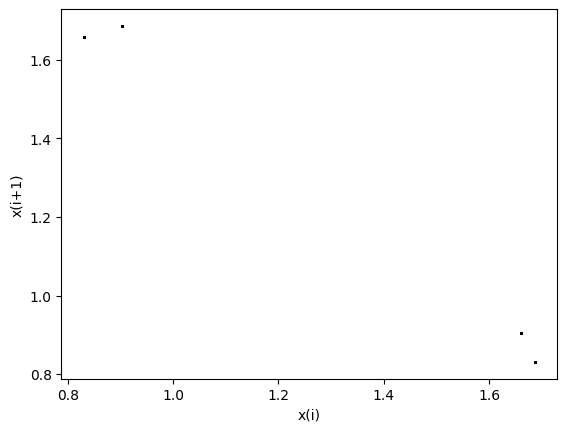
\includegraphics[width=\textwidth]{LateX images/graphs q03/g5}
		\caption{Για k=0.5}
		\label{f:k17}
	\end{subfigure}
	\hfill
	\begin{subfigure}[b]{0.25\textwidth}
		\centering
		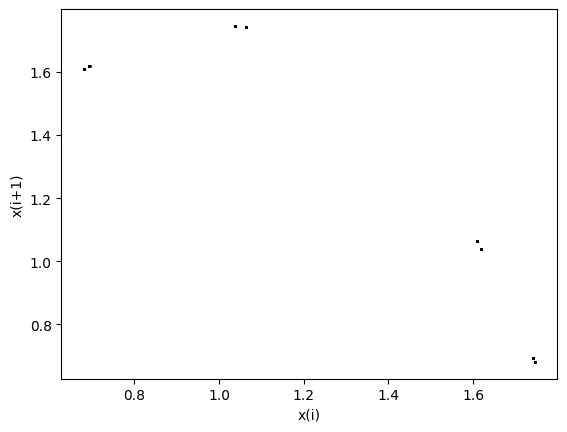
\includegraphics[width=\textwidth]{LateX images/graphs q03/g6}
		\caption{Για k=0.511}
		\label{f:k18}
	\end{subfigure}
	\hfill
	\begin{subfigure}[b]{0.25\textwidth}
		\centering
		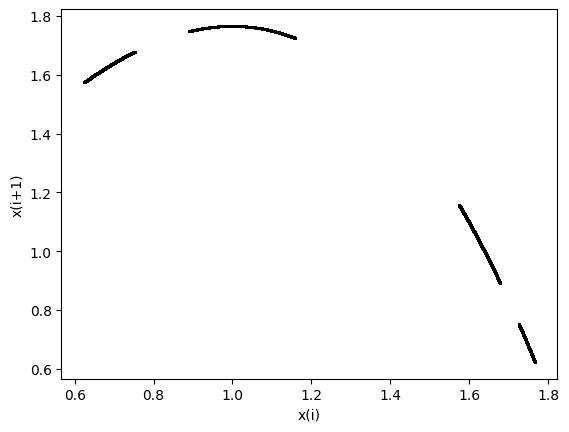
\includegraphics[width=\textwidth]{LateX images/graphs q03/g67}
		\caption{Για k=0.5165}
		\label{f:k19}
	\end{subfigure}
	\hfill
	\begin{subfigure}[b]{0.25\textwidth}
		\centering
		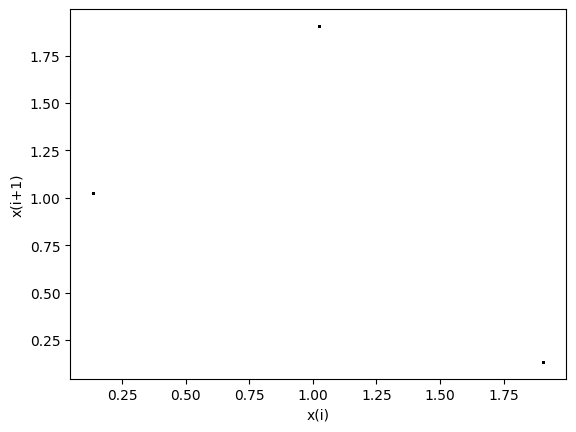
\includegraphics[width=\textwidth]{LateX images/graphs q03/g8}
		\caption{Για k=0.551}
		\label{f:k20}
	\end{subfigure}
	\hfill
	\begin{subfigure}[b]{0.25\textwidth}
		\centering
		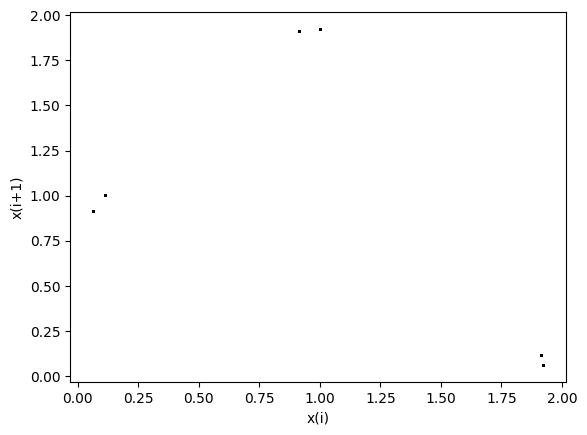
\includegraphics[width=\textwidth]{LateX images/graphs q03/g9}
		\caption{Για k=0.555}
		\label{f:k21}
	\end{subfigure}
	\hfill
	\begin{subfigure}[b]{0.25\textwidth}
		\centering
		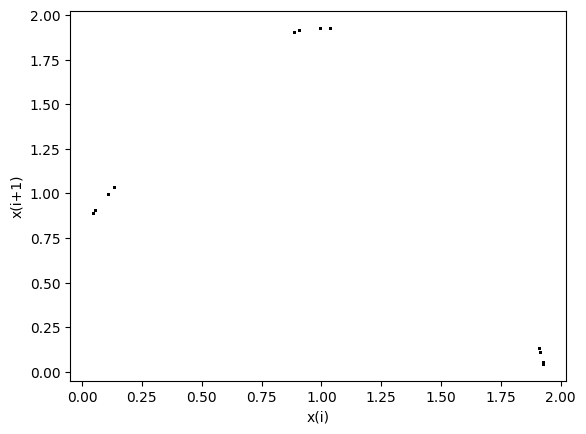
\includegraphics[width=\textwidth]{LateX images/graphs q03/g10}
		\caption{Για k=0.556}
		\label{f:k22}
	\end{subfigure}
	\hfill
	\begin{subfigure}[b]{0.25\textwidth}
		\centering
		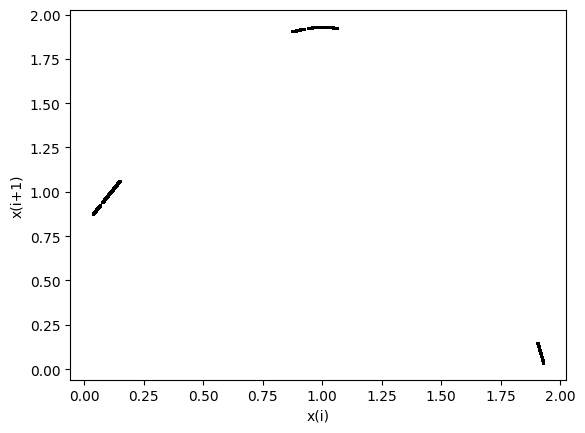
\includegraphics[width=\textwidth]{LateX images/graphs q03/g11}
		\caption{Για k=0.5573}
		\label{f:k23}
	\end{subfigure}
	\hfill
	\begin{subfigure}[b]{0.25\textwidth}
		\centering
		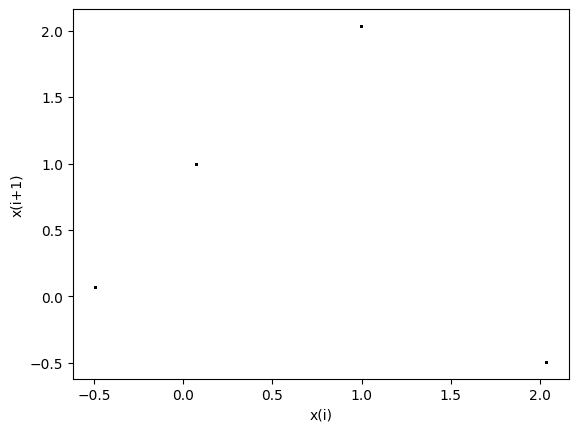
\includegraphics[width=\textwidth]{LateX images/graphs q03/g12}
		\caption{Για k=0.583}
		\label{f:k24}
	\end{subfigure}
	\hfill
	\begin{subfigure}[b]{0.25\textwidth}
		\centering
		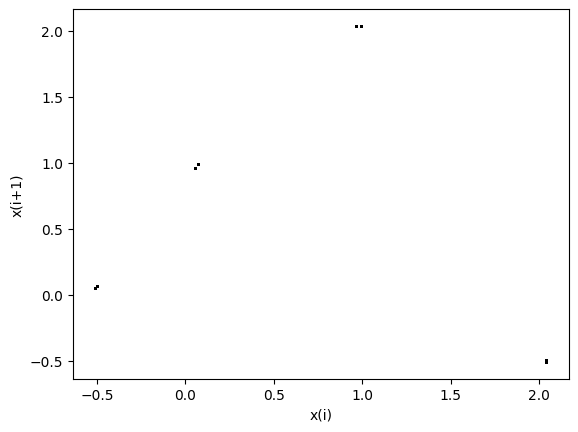
\includegraphics[width=\textwidth]{LateX images/graphs q03/g13}
		\caption{Για k=0.5846}
		\label{f:k25}
	\end{subfigure}
	\hfill
	\begin{subfigure}[b]{0.25\textwidth}
		\centering
		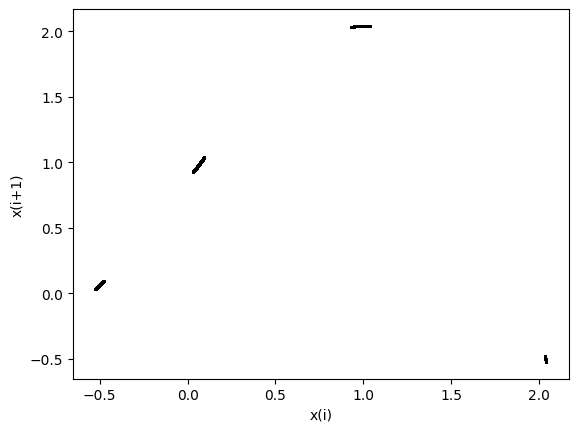
\includegraphics[width=\textwidth]{LateX images/graphs q03/g14}
		\caption{Για k=0.5851}
		\label{f:k26}
	\end{subfigure}
	
\end{figure}

\clearpage

\subsection{Για q=-0.5}

Στο σχήμα \ref{f:g10} παρατίθεται το διάγραμμα διακλάδωσης του συστήματος \ref{f:x1}, ως προς την παράμετρο k, για a=1, b=2 και q =- 0.5. Για αυτές τις τιμές των παραμέτρων το σύστημα ξεκινάει από περίοδο-1 για k = 0.3 , ενώ για  k = 0.48 εμφανίζει τον πρώτο διπλασιασμό της περιόδου. Τον δεύτερο διπλασιασμό τον εμφανίζει για k=0.53 (περίοδος-4) ,τον τρίτο για k=0.55 (περίοδος-8) και τον τέταρτο για k=0.5531 (περόδος-15).Στην συνέχεια για k>0.5534 το σύστημα εισέρχεται στο χάος , μέχρι να εξέλθει  για k=0.59(περίοδος-3) και να ξανά εισέλθει σε χάος μετά από δύο διπλασιασμούς k=0.59377 (περίοδος-6) ,για k>0.594.
Επομένως και σε αυτή την περίπτωση το σύστημα εισέρχεται στο χάος με διπλασιασμό της περιόδου. 
Επιπλέον, στο σχήμα \ref{f:g11} παρατίθεται το διάγραμμα των εκθετών Lyapunov για τιμές του k στο ίδιο διάστημα τιμών [0, 0.67].  Στο διάστημα τιμών   0<k<0.511 , στο 0.551<k<0.556, και στο 0.583<k<0.5846 παρατηρούμε ότι ο εκθέτης Lyapunov είναι συνεχώς αρνητικός, γεγονός που επιβεβαιώνει την περιοδική συμπεριφορά του συστήματος. Ενώ στα υπόλοιπα διαστήματα ο θετικός εκθέτης Lyapunov υποστηρίζει την χαοτική του συμπεριφορά, όπως έγινε φανερό και από το διάγραμμα διακλάδωσης.
Τέλος, στον Πίνακα \ref{tab:abc2} παρατίθενται ενδεικτικές τιμές της παραμέτρου k και η συμπεριφορά που παρουσιάζει το σύστημα για αυτές, σύμφωνα με το διάγραμμα διακλάδωσης, καθώς και τα αντίστοιχα σχήματα των διαγραμμάτων της τιμής \(x_i\) σε συνάρτηση με την τιμή \(x_{i+1}\). Από τα παραγόμενα σχήματα προκύπτει αριθμός σημείων αντίστοιχος με την περίοδο του συστήματος.

\begin{table}[h!]
	\centering
	\begin{tabular}{l | l | l}
		Παράμετρος k & Συμπεριφορά & Σχήμα\\
		\hline
		0.3 &  Περίοδος-1 & \ref{f:k1}\\
		0.48& Περίοδος-2 & \ref{f:k2}\\
		0.53& Περίοδος-4 & \ref{f:k2}\\
		0.55 &  Περίοδος-8 & \ref{f:k3}\\
		0.5531 & Περίοδος-15 & \ \\
		0.5534 & Χάος & \ref{f:k5}\\
		0.59 & Περίοδος-3 & \ref{f:k6})\\
		0.593 & Περίοδος-6 & \ref{f:k7}\\
		0.594 & Χάος & \ref{f:k9}\\
	\end{tabular}
	\caption{ Συμπεριφορά του υπό μελέτη συστήματος για διάφορες τιμές του k,για a=1, b=2 και q=-0.5}
	\label{tab:abc2}
\end{table}

\begin{figure}[h!]
	\centering
	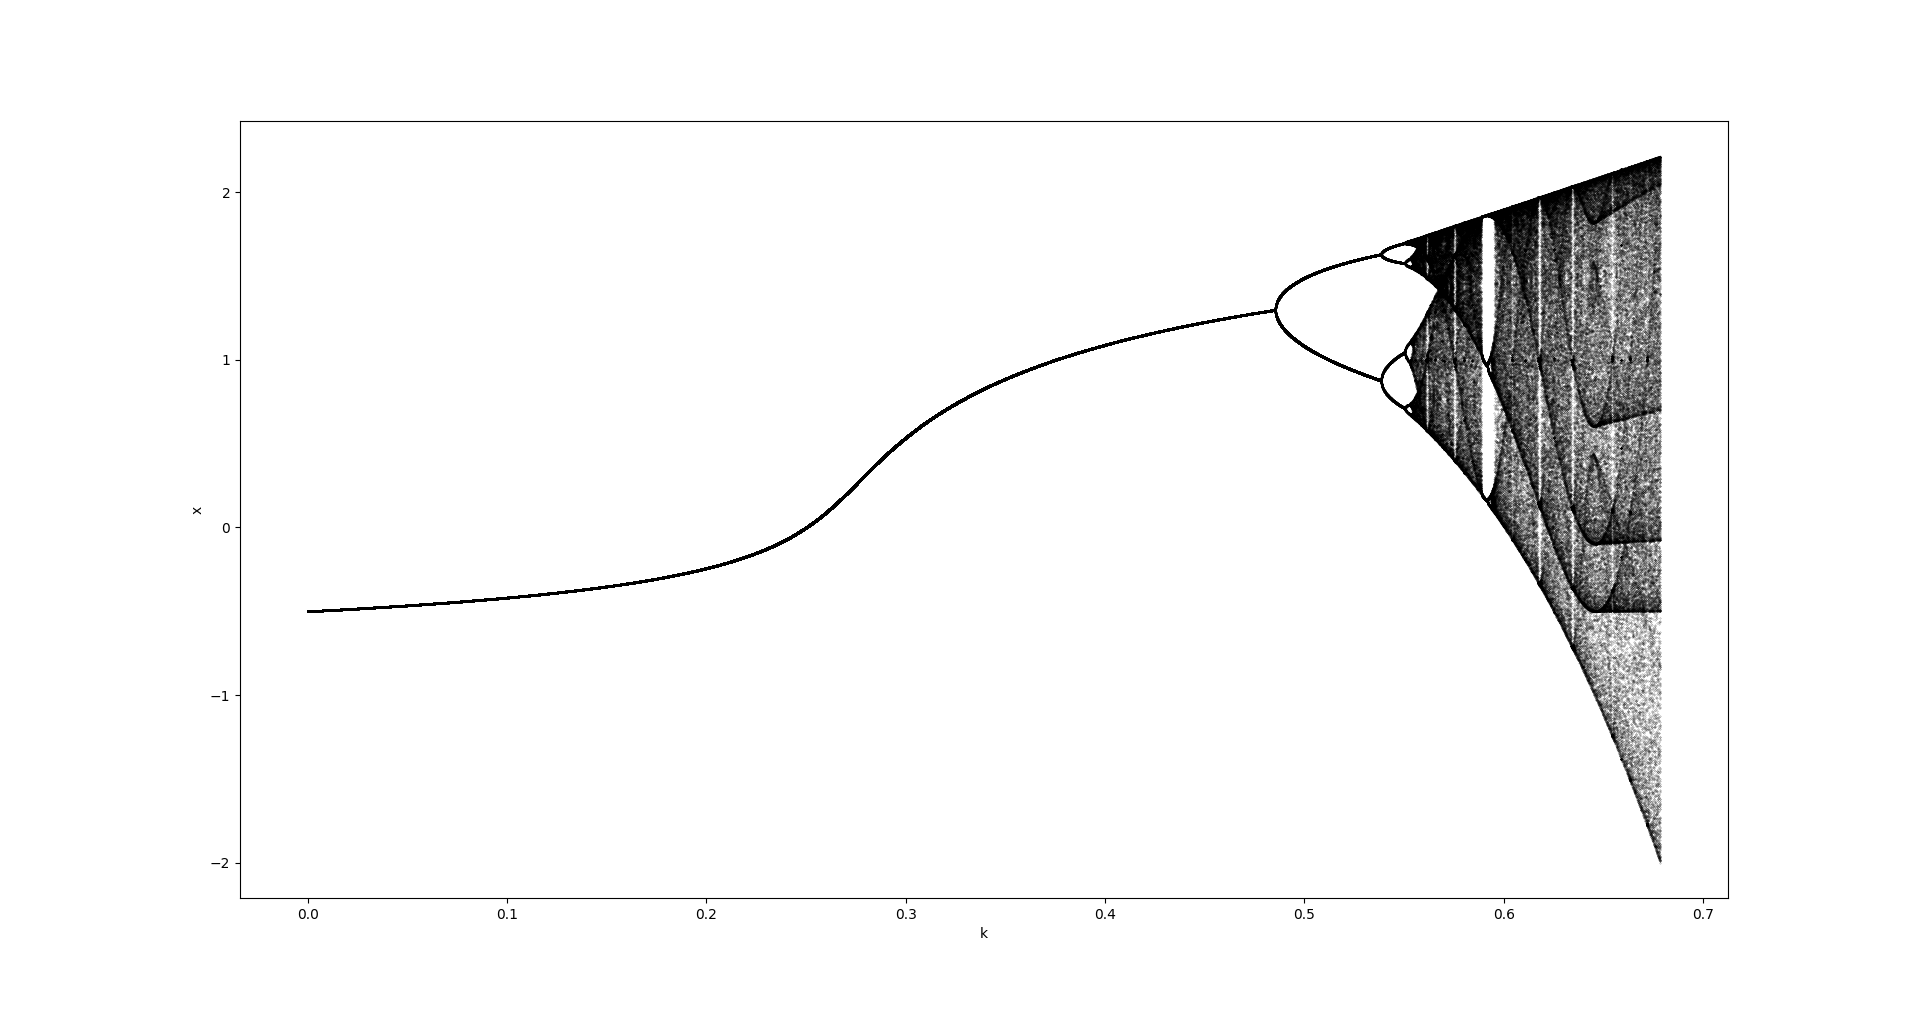
\includegraphics[width=0.6\linewidth]{LateX images/graphs q05/g1}
	\caption{ Διάγραμμα διακλάδωσης, για a=1, b=2 και q=-0.5}
	\label{f:g10}
\end{figure}

\begin{figure}[h!]
	\centering
	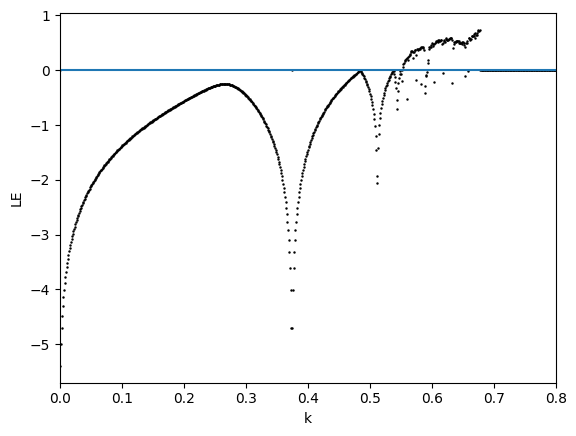
\includegraphics[width=0.6\linewidth]{LateX images/graphs q05/g2}
	\caption{ Διάγραμμα του εκθέτη Lyapunov σε συνάρτηση με την παράμετρο k, για a=1, b=2 και q=-0.5}
	\label{f:g11}
\end{figure}

\begin{figure}[h!]
	\centering
	\caption{Διαγράμματα της τιμής \(x_i\) με την τιμή \(x_{i+1}\) :}
	\begin{subfigure}[b]{0.25\textwidth}
		\centering
		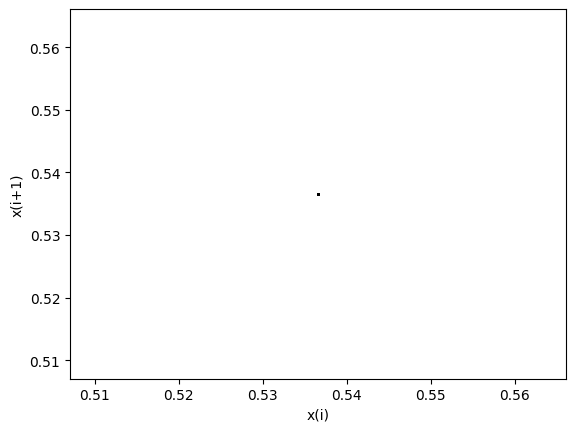
\includegraphics[width=\textwidth]{LateX images/graphs q05/g3}
		\caption{Για k=0.3}
		\label{f:k27}
	\end{subfigure}
	\hfill
	\begin{subfigure}[b]{0.25\textwidth}
		\centering
		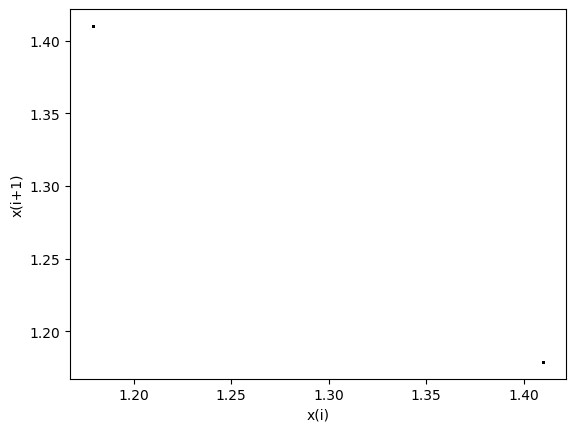
\includegraphics[width=\textwidth]{LateX images/graphs q05/g4}
		\caption{Για k=0.48}
		\label{f:k28}
	\end{subfigure}
	\hfill
	\begin{subfigure}[b]{0.25\textwidth}
		\centering
		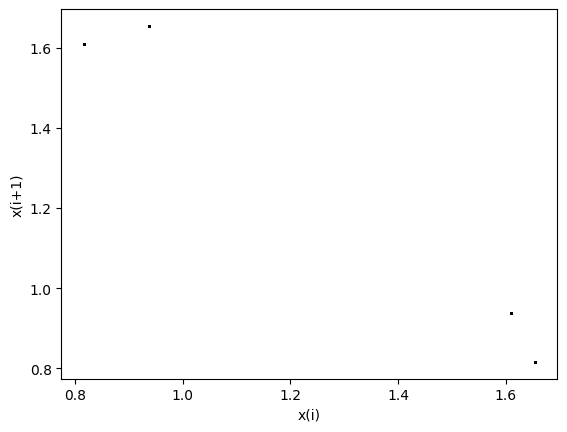
\includegraphics[width=\textwidth]{LateX images/graphs q05/g5}
		\caption{Για k=0.53}
		\label{f:k29}
	\end{subfigure}
	\begin{subfigure}[b]{0.25\textwidth}
		\centering
		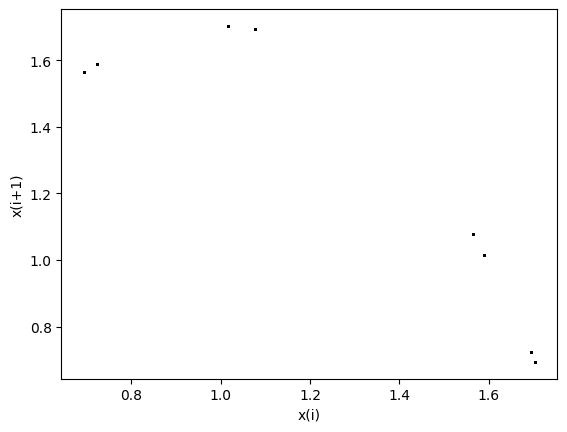
\includegraphics[width=\textwidth]{LateX images/graphs q05/g6}
		\caption{Για k=0.55}
		\label{f:k30}
	\end{subfigure}
	\hfill
	\begin{subfigure}[b]{0.25\textwidth}
		\centering
		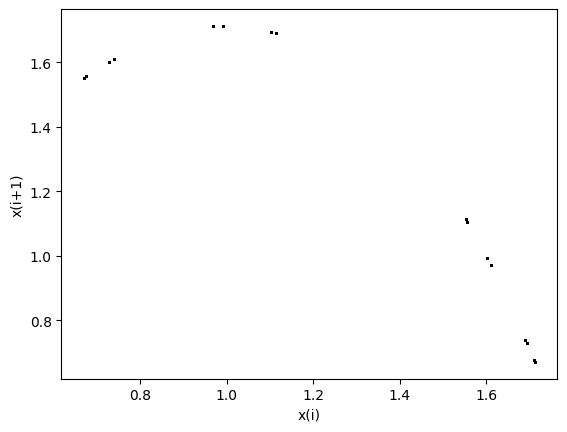
\includegraphics[width=\textwidth]{LateX images/graphs q05/g7}
		\caption{Για k=0.5531}
		\label{f:k31}
	\end{subfigure}
	\hfill
	\begin{subfigure}[b]{0.25\textwidth}
		\centering
		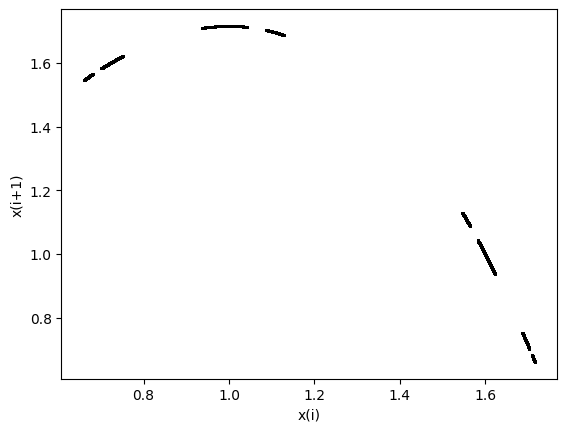
\includegraphics[width=\textwidth]{LateX images/graphs q05/g8}
		\caption{Για k=0.5534}
		\label{f:k32}
	\end{subfigure}
	\hfill
	\begin{subfigure}[b]{0.25\textwidth}
		\centering
		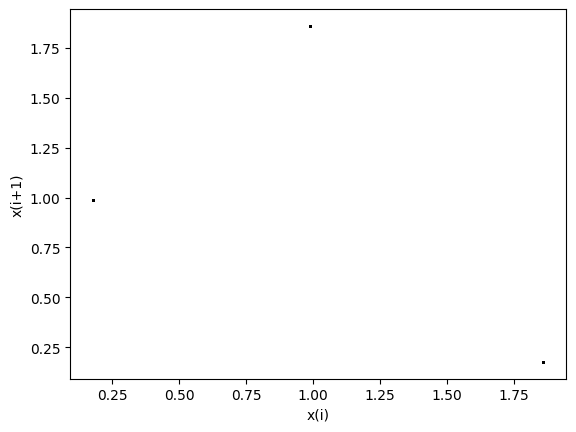
\includegraphics[width=\textwidth]{LateX images/graphs q05/g9}
		\caption{Για k=0.58}
		\label{f:k33}
	\end{subfigure}
	\hfill
	\begin{subfigure}[b]{0.25\textwidth}
		\centering
		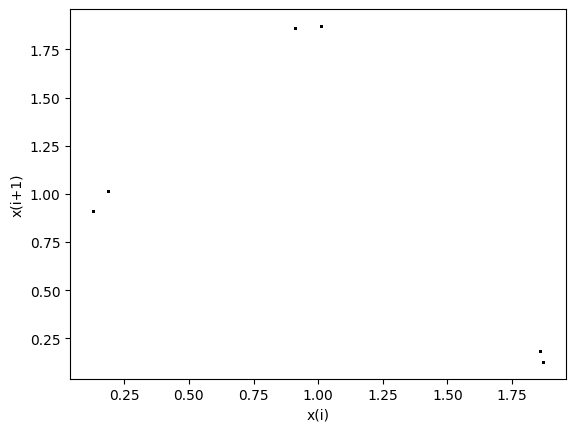
\includegraphics[width=\textwidth]{LateX images/graphs q05/g10}
		\caption{Για k=0.591}
		\label{f:k35}
	\end{subfigure}
	\hfill
	\begin{subfigure}[b]{0.25\textwidth}
		\centering
		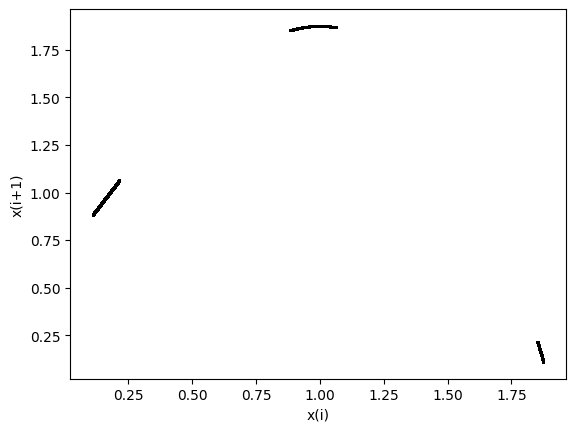
\includegraphics[width=\textwidth]{LateX images/graphs q05/g11}
		\caption{Για k=0.5927}
		\label{f:36}
	\end{subfigure}
		
\end{figure}

 \clearpage

\subsection{Για q=-0.7}

Στο σχήμα \ref{f:g12} παρατίθεται το διάγραμμα διακλάδωσης του συστήματος \ref{f:x1}, ως προς την παράμετρο k, για a=1, b=2 και q =- 0.7. Για αυτές τις τιμές των παραμέτρων το σύστημα ξεκινάει από περίοδο-1 για k = 0.3 αλλά από k[0.3469,0.3486] σπάει η περίοδος. Απο k=3.469 ξαναξεκινάει από περίοδο-1.Για  k = 0.52 εμφανίζει τον πρώτο διπλασιασμό της περιόδου. Τον δεύτερο διπλασιασμό τον εμφανίζει για k=0.57(περίοδος-4) ,τον τρίτο για k=0.592 (περίοδος-8) και τον τέταρτο για k=0.593(περόδος-15).Στην συνέχεια για k>0.593 το σύστημα εισέρχεται στο χάος , μέχρι να εξέλθει  για k=0.627(περίοδος-3) και να ξανά εισέλθει σε χάος μετά από δύο διπλασιασμούς k=0.63 (περίοδος-6)  k=0.631 (περίοδος-11),για k>0.631.
Επομένως και σε αυτή την περίπτωση το σύστημα εισέρχεται στο χάος με διπλασιασμό της περιόδου. 
Επιπλέον, στο σχήμα \ref{f:g11} παρατίθεται το διάγραμμα των εκθετών Lyapunov για τιμές του k στο ίδιο διάστημα τιμών [0, 0.72].  Στο διάστημα τιμών   0<k<0.594 , στο 0.627<k<0.632, παρατηρούμε ότι ο εκθέτης Lyapunov είναι συνεχώς αρνητικός, γεγονός που επιβεβαιώνει την περιοδική συμπεριφορά του συστήματος. Ενώ στα υπόλοιπα διαστήματα ο θετικός εκθέτης Lyapunov υποστηρίζει την χαοτική του συμπεριφορά, όπως έγινε φανερό και από το διάγραμμα διακλάδωσης.
Τέλος, στον Πίνακα \ref{tab:abc3} παρατίθενται ενδεικτικές τιμές της παραμέτρου k και η συμπεριφορά που παρουσιάζει το σύστημα για αυτές, σύμφωνα με το διάγραμμα διακλάδωσης, καθώς και τα αντίστοιχα σχήματα των διαγραμμάτων της τιμής \(x_i\) σε συνάρτηση με την τιμή \(x_{i+1}\). Από τα παραγόμενα σχήματα προκύπτει αριθμός σημείων αντίστοιχος με την περίοδο του συστήματος.

\begin{table}[h!]
	\centering
	\begin{tabular}{l | l | l}
		Παράμετρος k & Συμπεριφορά & Σχήμα\\
		\hline
		0.25 &  Περίοδος-1 & \ref{f:k37}\\
		0.3469&  Περίοδος-1 & \ref{f:k38}\\
		0.52& Περίοδος-2 & \ref{f:k39}\\
		0.57& Περίοδος-4 & \ref{f:k40}\\
		0.592 &  Περίοδος-8 & \ref{f:k41}\\
		0.593& Περίοδος-15 & \ref{f:k42}\\
		0.594 & Χάος & \ref{f:k43}\\
		0.627 & Περίοδος-3 & \ref{f:k44}\\
		0.630 & Περίοδος-6 & \ref{f:k45}\\
		0.631 & Περίοδος-11 & \ref{f:k46}\\
		0.632 & Χάος & \ref{f:k47}\\
	\end{tabular}
	\caption{ Συμπεριφορά του υπό μελέτη συστήματος για διάφορες τιμές του k,για a=1, b=2 και q=-0.7}
	\label{tab:abc3}
\end{table}

\begin{figure}[h!]
	\centering
	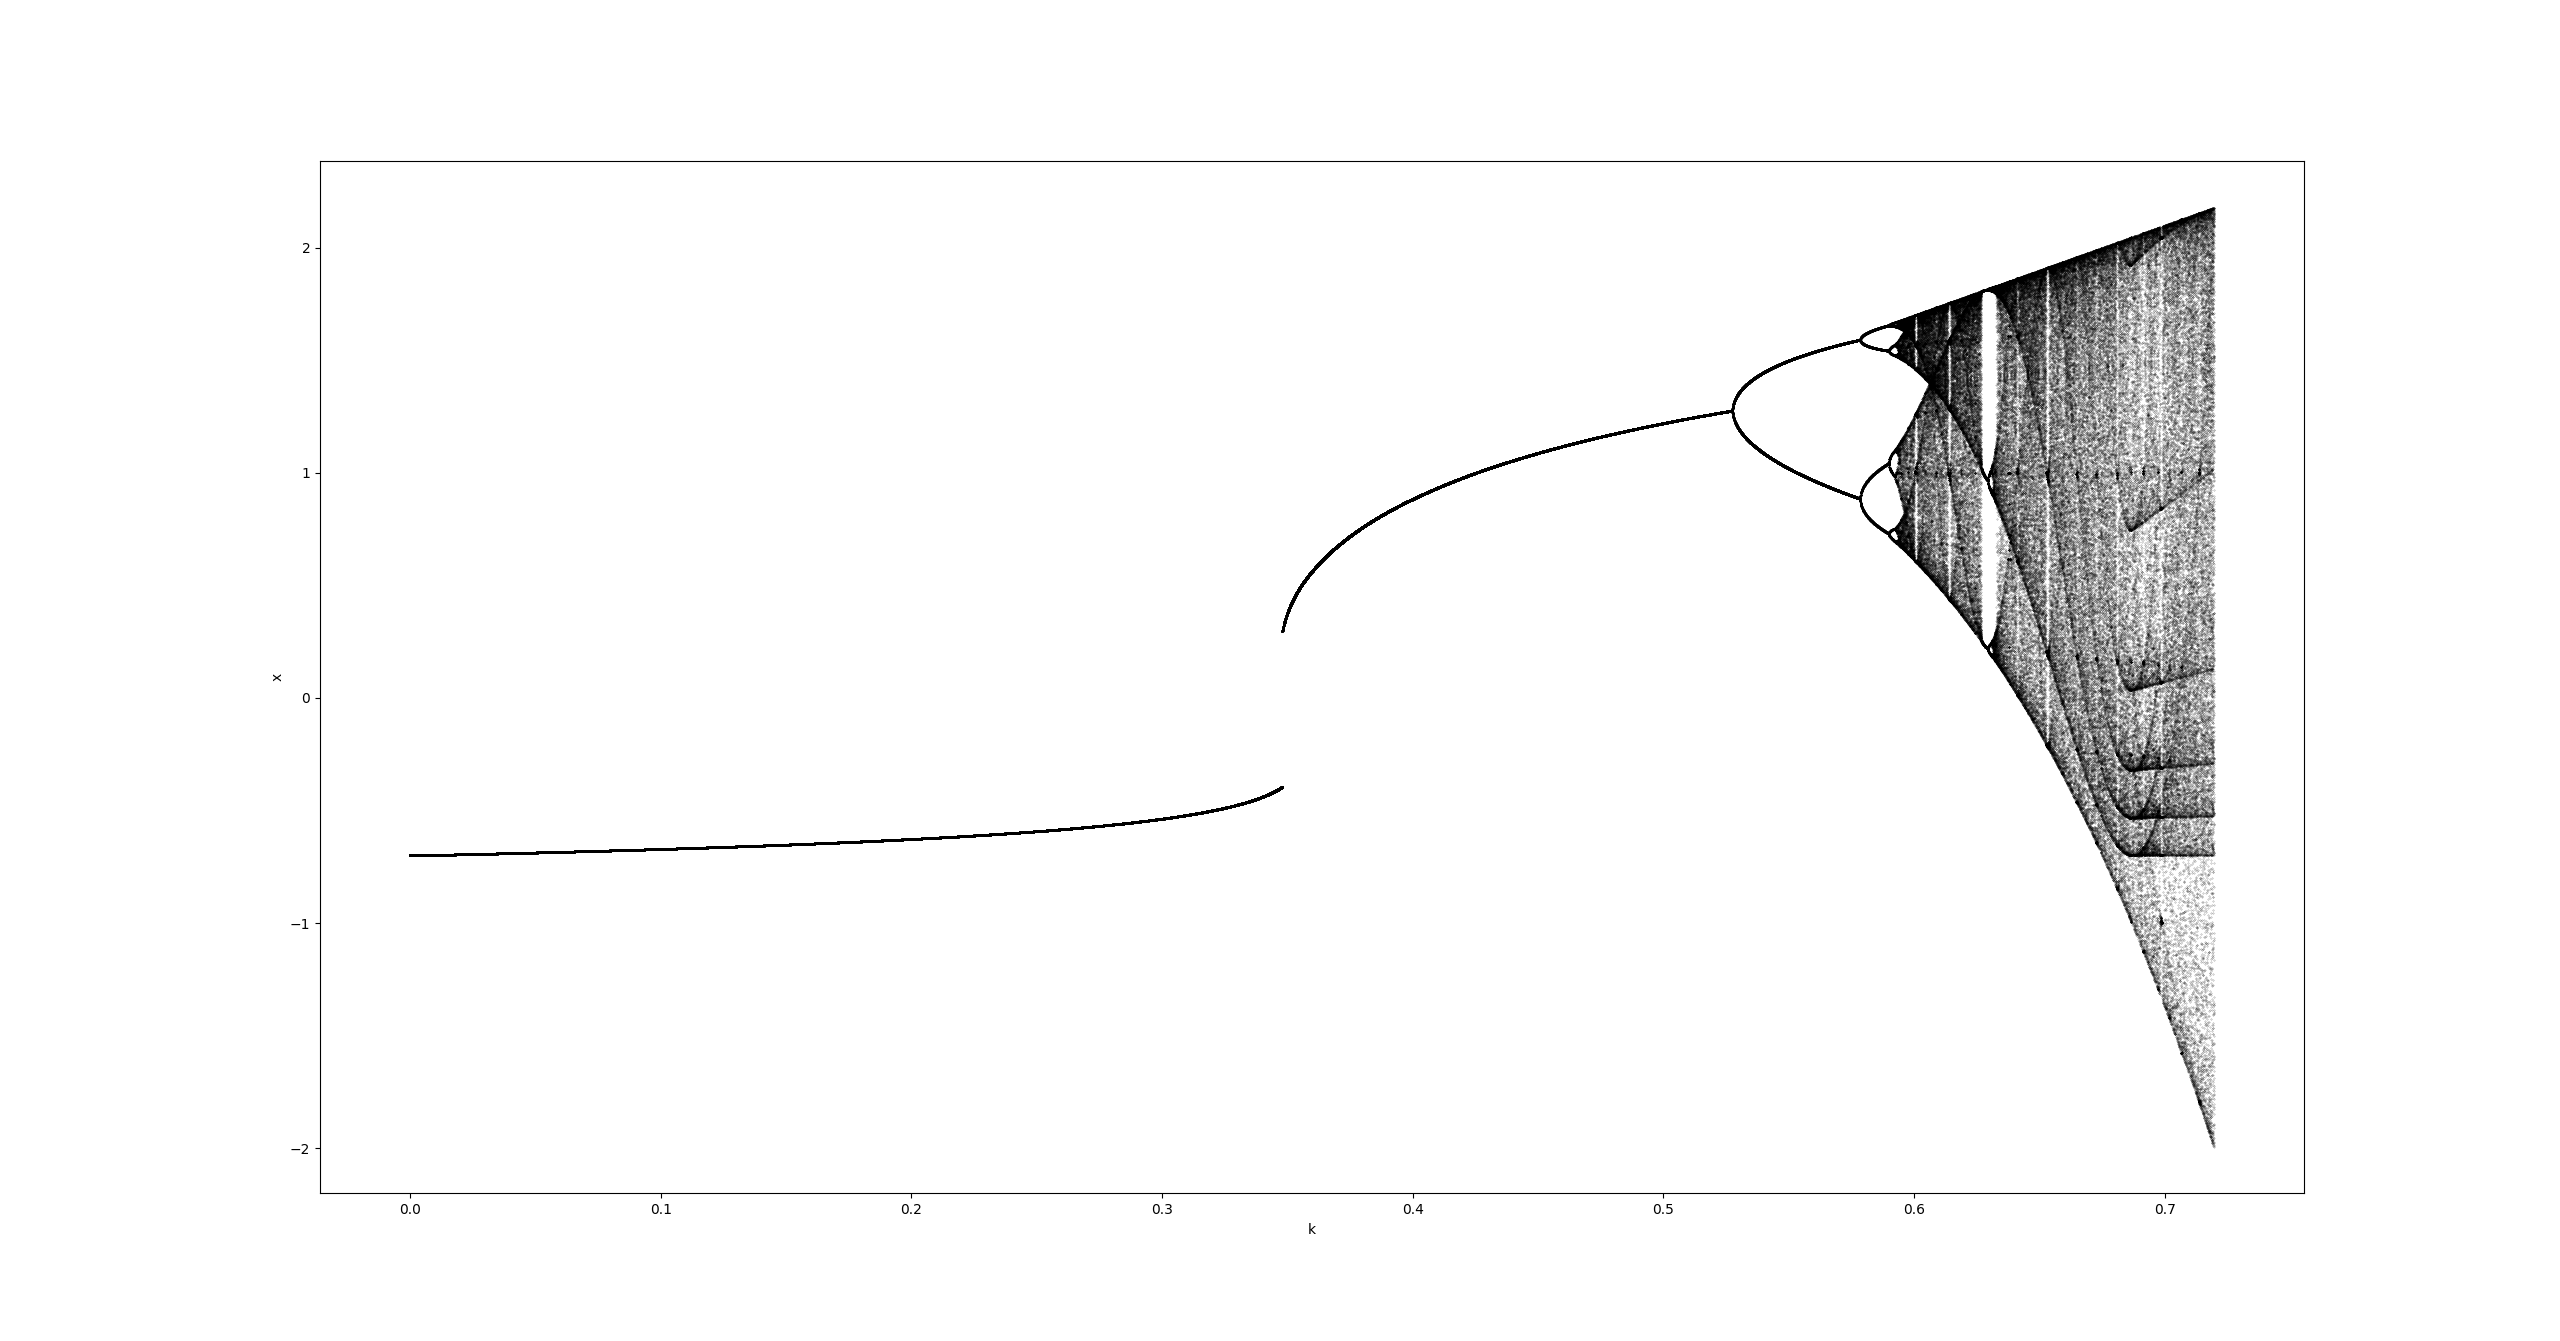
\includegraphics[width=0.6\linewidth]{LateX images/graphs q07/g1}
	\caption{ Διάγραμμα διακλάδωσης, για a=1, b=2 και q=-0.7}
	\label{f:g12}
\end{figure}
\begin{figure}[h!]
	\centering
	\includegraphics[width=0.6\linewidth]{"LateX images/graphs q07/g2 "}
	\caption{Διάγραμμα του εκθέτη Lyapunov σε συνάρτηση με την παράμετρο k, για a=1, b=2 και q=-0.7.}
	\label{f:g13}
\end{figure}

\begin{figure}[h!]
	\centering
	\caption{Διαγράμματα της τιμής \(x_i\) με την τιμή \(x_{i+1}\) :}
	\begin{subfigure}[b]{0.25\textwidth}
		\centering
		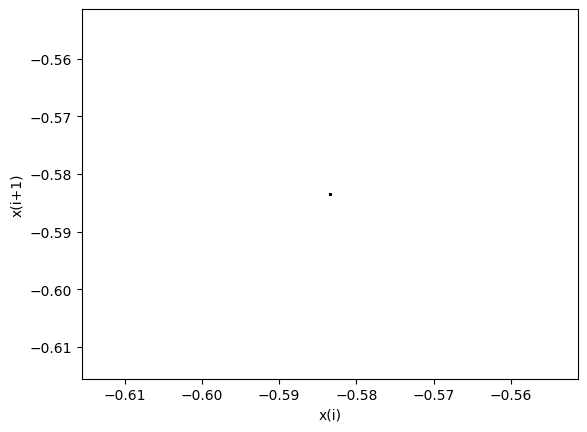
\includegraphics[width=\textwidth]{LateX images/graphs q07/g3}
		\caption{Για k=0.25}
		\label{f:k37}
	\end{subfigure}
	\hfill
	\begin{subfigure}[b]{0.25\textwidth}
		\centering
		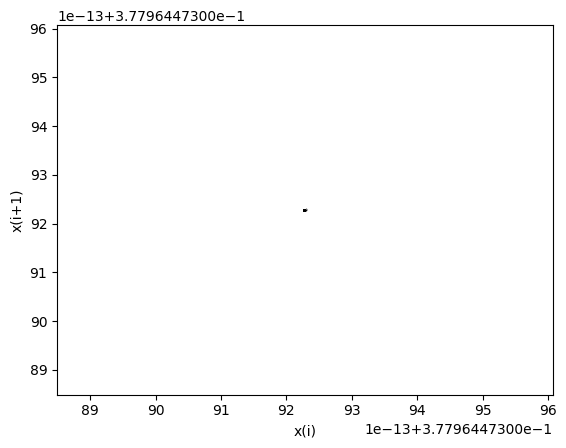
\includegraphics[width=\textwidth]{LateX images/graphs q07/g4}
		\caption{Για k=0.3469}
		\label{f:k38}
	\end{subfigure}
	\hfill
	\begin{subfigure}[b]{0.25\textwidth}
		\centering
		\includegraphics[width=\textwidth]{LateX images/graphs q07/g5}
		\caption{Για k=0.52}
		\label{f:k39}
	\end{subfigure}
	\begin{subfigure}[b]{0.25\textwidth}
		\centering
		\includegraphics[width=\textwidth]{LateX images/graphs q07/g6}
		\caption{Για k=0.57}
		\label{f:k40}
	\end{subfigure}
	\hfill
	\begin{subfigure}[b]{0.25\textwidth}
		\centering
		\includegraphics[width=\textwidth]{LateX images/graphs q07/g7}
		\caption{Για k=0.592}
		\label{f:k41}
	\end{subfigure}
	\hfill
	\begin{subfigure}[b]{0.25\textwidth}
		\centering
		\includegraphics[width=\textwidth]{LateX images/graphs q07/g8}
		\caption{Για k=0.593}
		\label{f:k42}
	\end{subfigure}
	\hfill
	\begin{subfigure}[b]{0.25\textwidth}
		\centering
		\includegraphics[width=\textwidth]{LateX images/graphs q07/g9}
		\caption{Για k=0.594}
		\label{f:k43}
	\end{subfigure}
	\hfill
	\begin{subfigure}[b]{0.25\textwidth}
		\centering
		\includegraphics[width=\textwidth]{LateX images/graphs q07/g10}
		\caption{Για k=0.627}
		\label{f:k44}
	\end{subfigure}
	\hfill
	\begin{subfigure}[b]{0.25\textwidth}
		\centering
		\includegraphics[width=\textwidth]{LateX images/graphs q07/g11}
		\caption{Για k=0.63}
		\label{f:k45}
	\end{subfigure}
	\hfill
	\begin{subfigure}[b]{0.25\textwidth}
		\centering
		\includegraphics[width=\textwidth]{LateX images/graphs q07/g12}
		\caption{Για k=0.631}
		\label{f:k46}
	\end{subfigure}
	\hfill
	\begin{subfigure}[b]{0.25\textwidth}
	\centering
	\includegraphics[width=\textwidth]{LateX images/graphs q07/g13}
	\caption{Για k=0.632}
	\label{f:k47}
	\end{subfigure}
	
\end{figure}

\clearpage

\subsection{Για q=-0.9}

\begin{table}[h!]
	\centering
	\begin{tabular}{l | l | l}
		Παράμετρος k & Συμπεριφορά & Σχήμα\\
		\hline
		0.43 &  Περίοδος-1 & \ref{f:k48}\\
		0.436 &  Περίοδος-1 & \ref{f:k49}\\
		0.57& Περίοδος-2 & \ref{f:k50}\\
		0.62& Περίοδος-4 & \ref{f:k51}\\
		0.63 &  Περίοδος-8 & \ref{f:k52}\\
		0.633& Περίοδος-16 & \ref{f:k53}\\
		0.635& Χάος & \ref{f:k54}\\
		0.665 & Περίοδος-3 & \ref{f:k55}\\
		0.668 & Περίοδος-6 & \ref{f:k56}\\
		0.671 & Χάος & \ref{f:k57}\\
		0.72 & Περίοδος-1& \ref{f:k58}\\
	\end{tabular}
	\caption{ Συμπεριφορά του υπό μελέτη συστήματος για διάφορες τιμές του k,για a=1, b=2 και q=-0.9}
	\label{tab:abc4}
\end{table}

\begin{figure}[h!]
	\centering
	\includegraphics[width=0.6\linewidth]{LateX images/graphs q09/g1}
	\caption{ Διάγραμμα διακλάδωσης, για a=1, b=2 και q=-0.9}
	\label{f:g14}
\end{figure}

\begin{figure}[h!]
	\centering
	\includegraphics[width=0.6\linewidth]{LateX images/graphs q09/g2}
	\caption{Διάγραμμα του εκθέτη Lyapunov σε συνάρτηση με την παράμετρο k, για a=1, b=2 και q=-0.9}
	\label{f:g15}
\end{figure}

\begin{figure}[h!]
	\centering
	\caption{Διαγράμματα της τιμής \(x_i\) με την τιμή \(x_{i+1}\) :}
	\begin{subfigure}[b]{0.25\textwidth}
		\centering
		\includegraphics[width=\textwidth]{LateX images/graphs q09/g3}
		\caption{Για k=0.43}
		\label{f:k48}
	\end{subfigure}
	\hfill
	\begin{subfigure}[b]{0.25\textwidth}
		\centering
		\includegraphics[width=\textwidth]{LateX images/graphs q09/g4}
		\caption{Για k=0.436}
		\label{f:k49}
	\end{subfigure}
	\hfill
	\begin{subfigure}[b]{0.25\textwidth}
		\centering
		\includegraphics[width=\textwidth]{LateX images/graphs q09/g5}
		\caption{Για k=0.57}
		\label{f:k50}
	\end{subfigure}
	\begin{subfigure}[b]{0.25\textwidth}
		\centering
		\includegraphics[width=\textwidth]{LateX images/graphs q09/g6}
		\caption{Για k=0.62}
		\label{f:k51}
	\end{subfigure}
	\hfill
	\begin{subfigure}[b]{0.25\textwidth}
		\centering
		\includegraphics[width=\textwidth]{LateX images/graphs q09/g13}
		\caption{Για k=0.63}
		\label{f:k52}
	\end{subfigure}
	\hfill
	\begin{subfigure}[b]{0.25\textwidth}
		\centering
		\includegraphics[width=\textwidth]{LateX images/graphs q09/g7}
		\caption{Για k=0.633}
		\label{f:k53}
	\end{subfigure}
	\hfill
	\begin{subfigure}[b]{0.25\textwidth}
		\centering
		\includegraphics[width=\textwidth]{LateX images/graphs q09/g8}
		\caption{Για k=0.635}
		\label{f:k54}
	\end{subfigure}
	\hfill
	\begin{subfigure}[b]{0.25\textwidth}
		\centering
		\includegraphics[width=\textwidth]{LateX images/graphs q09/g9}
		\caption{Για k=0.665}
		\label{f:k55}
	\end{subfigure}
	\hfill
	\begin{subfigure}[b]{0.25\textwidth}
		\centering
		\includegraphics[width=\textwidth]{LateX images/graphs q09/g10}
		\caption{Για k=0.668}
		\label{f:k56}
	\end{subfigure}
	\hfill
	\begin{subfigure}[b]{0.25\textwidth}
		\centering
		\includegraphics[width=\textwidth]{LateX images/graphs q09/g11}
		\caption{Για k=0.671}
		\label{f:k57}
	\end{subfigure}
	\hfill
	\begin{subfigure}[b]{0.25\textwidth}
		\centering
		\includegraphics[width=\textwidth]{LateX images/graphs q09/g12}
		\caption{Για k=0.72}
		\label{f:k58}
	\end{subfigure}
	\hfill
	
\end{figure}

\clearpage

\subsection{Για q=-1.2}

\begin{table}[h!]
	\centering
	\begin{tabular}{l | l | l}
		Παράμετρος k & Συμπεριφορά & Σχήμα\\
		\hline
		0.55 &  Περίοδος-1 & \ref{f:k59}\\
		0.566 &  Περίοδος-1 & \ref{f:k60}\\
		0.63& Περίοδος-2 & \ref{f:k61}\\
		0.68& Περίοδος-4 & \ref{f:k62}\\
		0.69 &  Περίοδος-8 & \ref{f:k63}\\
		0.696& Χάος & \ref{f:k64}\\
		0.726& Περίοδος-3 & \ref{f:k65}\\
		0.729& Περίοδος-6 & \ref{f:k66}\\
		0.731& Χάος & \ref{f:k67}\\
		0.762 &  Περίοδος-1 & \ref{f:k68}\\
	\end{tabular}
	\caption{ Συμπεριφορά του υπό μελέτη συστήματος για διάφορες τιμές του k,για a=1, b=2 και q=-0.9}
	\label{tab:abc5}
\end{table}

\begin{figure}[h!]
	\centering
	\includegraphics[width=0.6\linewidth]{LateX images/graphs q12/g1}
	\caption{ Διάγραμμα διακλάδωσης, για a=1, b=2 και q=-1.2}
	\label{f:g16}
\end{figure}

\begin{figure}[h!]
	\centering
	\includegraphics[width=0.6\linewidth]{LateX images/graphs q12/g2}
	\caption{Διάγραμμα του εκθέτη Lyapunov σε συνάρτηση με την παράμετρο k, για a=1, b=2 και q=-1.2}
	\label{f:g17}
\end{figure}

\begin{figure}[h!]
	\centering
	\caption{Διαγράμματα της τιμής \(x_i\) με την τιμή \(x_{i+1}\) :}
	\begin{subfigure}[b]{0.25\textwidth}
		\centering
		\includegraphics[width=\textwidth]{LateX images/graphs q12/g3}
		\caption{Για k=0.55}
		\label{f:k59}
	\end{subfigure}
	\hfill
	\begin{subfigure}[b]{0.25\textwidth}
		\centering
		\includegraphics[width=\textwidth]{LateX images/graphs q12/g4}
		\caption{Για k=0.566}
		\label{f:k60}
	\end{subfigure}
	\hfill
	\begin{subfigure}[b]{0.25\textwidth}
		\centering
		\includegraphics[width=\textwidth]{LateX images/graphs q12/g5}
		\caption{Για k=0.63}
		\label{f:k61}
	\end{subfigure}
	\begin{subfigure}[b]{0.25\textwidth}
		\centering
		\includegraphics[width=\textwidth]{LateX images/graphs q12/g6}
		\caption{Για k=0.68}
		\label{f:k62}
	\end{subfigure}
	\hfill
	\begin{subfigure}[b]{0.25\textwidth}
		\centering
		\includegraphics[width=\textwidth]{LateX images/graphs q12/g7}
		\caption{Για k=0.69}
		\label{f:k63}
	\end{subfigure}
	\hfill
	\begin{subfigure}[b]{0.25\textwidth}
		\centering
		\includegraphics[width=\textwidth]{LateX images/graphs q12/g8}
		\caption{Για k=0.696}
		\label{f:k64}
	\end{subfigure}
	\hfill
	\begin{subfigure}[b]{0.25\textwidth}
		\centering
		\includegraphics[width=\textwidth]{LateX images/graphs q12/g9}
		\caption{Για k=0.726}
		\label{f:k65}
	\end{subfigure}
	\hfill
	\begin{subfigure}[b]{0.25\textwidth}
		\centering
		\includegraphics[width=\textwidth]{LateX images/graphs q12/g10}
		\caption{Για k=0.729}
		\label{f:k66}
	\end{subfigure}
	\hfill
	\begin{subfigure}[b]{0.25\textwidth}
		\centering
		\includegraphics[width=\textwidth]{LateX images/graphs q12/g11}
		\caption{Για k=0.731}
		\label{f:k67}
	\end{subfigure}
	\hfill
	\begin{subfigure}[b]{0.25\textwidth}
		\centering
		\includegraphics[width=\textwidth]{LateX images/graphs q12/g12}
		\caption{Για k=0.762}
		\label{f:k68}
	\end{subfigure}
	\hfill
	
\end{figure}

\clearpage

\subsection{Για q=-1.4}

\begin{table}[h!]
	\centering
	\begin{tabular}{l | l | l}
		Παράμετρος k & Συμπεριφορά & Σχήμα\\
		\hline
		0.5 &  Περίοδος-1 & \ref{f:k59}\\
		0.54 &  Περίοδος-2 & \ref{f:k60}\\
		0.65& Περίοδος-1 & \ref{f:k61}\\
		0.68& Περίοδος-2 & \ref{f:k62}\\
		0.725 &  Περίοδος-4 & \ref{f:k63}\\
		0.735& Περίοδος-8 & \ref{f:k64}\\
		0.737& Περίοδος-15 & \ref{f:k65}\\
		0.738& Χάος & \ref{f:k66}\\
		0.767 &  Περίοδος-3& \ref{f:k68}\\
		0.769 &  Περίοδος-6& \ref{f:k68}\\
		0.77 &  Χάος& \ref{f:k68}\\
		0.8 &  Περίοδος-2& \ref{f:k68}\\
		
	\end{tabular}
	\caption{ Συμπεριφορά του υπό μελέτη συστήματος για διάφορες τιμές του k,για a=1, b=2 και q=-0.9}
	\label{tab:abc6}
\end{table}

[0,0.91]
